\section{Discussion}

\subsection{Multiple Measurements}
 Sequence flip of measurements step is the major factor that affects the localization performance.
 However, in some cases, sequence flip may provide more tight constraints to sequence-based localization when multiple TOA measurements are taken. 
 When the position of two nodes in the node sequence is subject to flip during multiple measurements, 
 it means that the TOA measurements of two nodes is very close,  the acoustic source is near to the perpendicular bisector of two nodes.
In this case, the distances from the acoustic source to the two node are nearly equal:
   \begin{equation} \label{12}
 \left\| {d_i - d_j } \right\| \le \epsilon_{ij}
  \end{equation}
 where $\epsilon_{ij}$ is the threshold parameter. Inequality \eqref{12} is equivalent to the following two linear constraints

 \begin{eqnarray} \label{13}
 \begin{array}{l}
 d_i - d_j \le \epsilon_{ij}  \\
 d_j - d_i \le \epsilon_{ij}  \\
  \end{array}
 \end{eqnarray}



 % \subsection{the uncertainty of the measurement}
% % Linear Programming with Probability Constraints - Part 1
% % Chance Constrained Programming
% % Cutting-plane
% %k-Violation linear programming
 % Considering the uncertainty of the TOA measurement,
 % Given the following node sequence $NodeSeq( \cdots ,i,j, \cdots )$, the uncertainty of ${d_i} < {d_j}$ can be described as : 
 % \begin{equation}
 % p({d_i} < {d_j})>\alpha
 % \end{equation}
 %where ${x_i,y_i}$ and ${x_j,y_j}$ are modelled as independent random variables following the normal distribution with the known parameter in the inequality.




\subsection{Time Synchronization }

For the sake of presentation, we assume that accurate time synchronization is achieved in the sensor network in the proposed LPSDL system.
Because TOA measurements are ultilized to achieve the node sequence, time synchronization is also an important factor to affect the localization performance. 
In this section, we disscuss the effect of time synchronization in acoustic sensor network.
Like the effect of TOA detection error, time synchronization error maybe also occur flip problem when computing the node sequence in LPSBL system, then lead to localization error.
Traditional time synchronization protocol, such as RBS, TPSN, and FTSP, can achieve synchronization less than 100ns. 
Compared with the the measurement error of TOA, time synchronization error has little effect on the LPSBL system.

% \subsection{Multiple Source Localization}

% Localizing multiple, simultaneously active sources is a more difficult problem. 
% In order to avoid conflict of several source, multiple source localization must be able to uniquely identify the signature of each acoustic source, which is beyond the capability of this paper. 
% So we will not do too much discussion about it in this paper.
% We just take an example, if the several targets are set as shown in Fig. 3, then we can calculate the location of the targets 
% because the acoustic source I is far enough from source II and the single from them can be distinguished. 
% So the smartphones close to the area I could handle the source I, and another smartphones close to the area II could handle the source II. 
% The Fig. 3 also describes system scalability.
% We can use a range to divide the large-scale area into to a smaller area that is large enough to cover the coverage of the acoustic source's signal.
% And the small area can be handled as our algorithm proposed by preceding part of the paper.

% %  \label必须放在\caption命令的后面
  % \begin{figure}[ht]
            % \setlength{\abovecaptionskip}{0pt}
            % \centering
            % 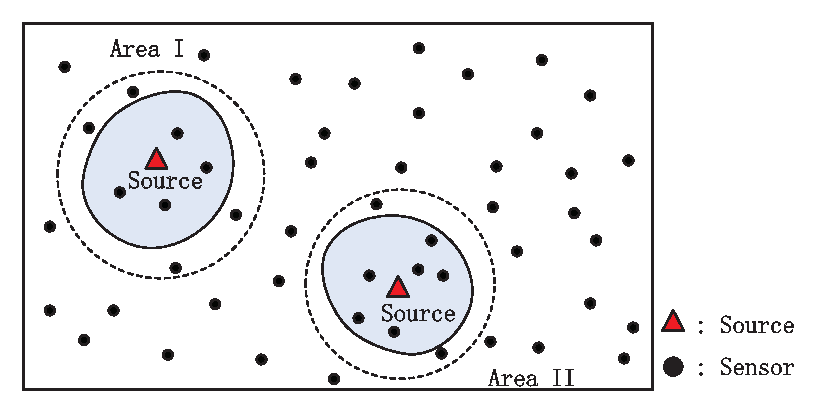
\includegraphics[scale=1.4,height=4.0cm]{image/fig3.eps}
             % \vspace{1mm}
			% \caption{Scalability for large-scale system}
			% \label{Fig3}
            % \label{multiple_source_localization}
            % \vspace{-5mm}
  % \end{figure}


% \subsection{Energy Efficiency}
% Energy efficiency is another issue in distributed acoustic sensor networks.
% Most of the time, acoustic sensor nodes keep asleep until the acoustic source appears in its sensing area.  
% The smartphone nodes near the acoustic source detect the acoustic signal, then alert its neighbour smartphones to prepare for receiving the signal.
% In this way, the proposed LPSBL system can save energy of acoustic sensors, then prolong the service life of distributed acoustic sensor networks.







